\documentclass[11pt,a4paper,twocolumn]{article}

% ── Packages ─────────────────────────────────────────────────────
\usepackage{times}
\usepackage{microtype}
\usepackage{geometry}
\geometry{a4paper, top=1in, bottom=1in, left=0.75in, right=0.75in, columnsep=0.25in}
\usepackage{titlesec}
\usepackage{booktabs}
\usepackage{url}
\usepackage[hidelinks]{hyperref}
\usepackage{natbib}
\usepackage{amsmath,amssymb}
\usepackage{graphicx}
\usepackage{enumitem}
\usepackage{algorithm}
\usepackage{algpseudocode}
\usepackage{tikz}
\usetikzlibrary{arrows.meta, positioning}
\usepackage{array}
\usepackage{filecontents}
\usepackage{authblk}

% ── Section formatting ───────────────────────────────────────────
\titleformat{\section}{\normalfont\bfseries}{\thesection}{0.5em}{}
\titleformat{\subsection}{\normalfont\bfseries\itshape}{\thesubsection}{0.5em}{}
\titlespacing{\section}{0pt}{8pt}{3pt}
\titlespacing{\subsection}{0pt}{5pt}{2pt}

\setlength{\parindent}{0pt}
\setlength{\parskip}{4pt}

% ── Embedded bibliography ────────────────────────────────────────
\begin{filecontents}{refs_spanner.bib}

@inproceedings{chimani2022spanner,
  author    = {Markus Chimani and Finn Stutzenstein},
  title     = {Spanner Approximations in Practice},
  booktitle = {30th Annual European Symposium on Algorithms ({ESA} 2022)},
  series    = {Leibniz International Proceedings in Informatics ({LIPIcs})},
  volume    = {244},
  pages     = {37:1--37:15},
  publisher = {Schloss Dagstuhl -- Leibniz-Zentrum f{\"u}r Informatik},
  address   = {Dagstuhl, Germany},
  year      = {2022},
  doi       = {10.4230/LIPIcs.ESA.2022.37}
}

\end{filecontents}

% ── Title block ──────────────────────────────────────────────────
\title{\textbf{Graph Spanner Approximations in Practice:
Engineering and Benchmarking Sparse Distance-Preserving Subgraphs}}

\author[1]{Sheikh Muhammad Muneeb \quad Abdul Moiz Ahmed \quad Moosa Owais}
\affil[1]{Habib University, Karachi\\
\small\texttt{\{ms08914, aa08811, mo08952\}@st.habib.edu.pk}}
\date{11 March 2026}

\begin{document}
\maketitle

% ── Abstract ─────────────────────────────────────────────────────
\begin{abstract}
This proposal outlines the implementation and empirical evaluation
of two graph spanner construction algorithms, as studied by
Chimani and Stutzenstein (2022) in ESA 2022.
A multiplicative $\alpha$-spanner is a sparse subgraph that
preserves all pairwise distances within a factor of~$\alpha$.
We implement the classical Greedy algorithm and the
randomized Baswana--Sen clustering algorithm, evaluating them
on synthetic and real-world networks with respect to running time,
sparseness, lightness, and effective stretch.
\end{abstract}

% ── 1. Introduction ──────────────────────────────────────────────
\section{Introduction and Problem Selection}

The chosen project follows Option~A: Paper-Based Implementation.
We have selected the paper ``Spanner Approximations in Practice''
published in the 30th Annual European Symposium on Algorithms
(ESA~2022), Track~B (Engineering and Applications)
\citep{chimani2022spanner}.

A \emph{multiplicative $\alpha$-spanner} $H$ of a weighted
undirected graph $G = (V, E)$ is a subgraph $H \subseteq G$
that satisfies $d_H(u,v) \leq \alpha \cdot d_G(u,v)$
for all $u, v \in V$, where $d_G$ denotes shortest-path distance.
The goal is to construct such an $H$ with as few edges as possible.
Spanners have direct applications in routing, network design,
distributed computing, and approximate distance oracles,
as surveyed in \citet{chimani2022spanner}.

Despite the existence of many spanner algorithms with strong
theoretical guarantees, no systematic experimental comparison
existed prior to \citet{chimani2022spanner}. Their paper fills
this gap by implementing and benchmarking multiple algorithms
on diverse graph families. We focus on the two most accessible
algorithms in that study: the Greedy spanner and the
Baswana--Sen (BS) clustering algorithm.

% ── 2. Brief Summary ─────────────────────────────────────────────
\section{Brief Summary of Research Contribution}

The primary contribution of \citet{chimani2022spanner} is the
first comprehensive experimental study of multiplicative spanner
approximation algorithms.
The paper implements and evaluates five algorithms across three
graph libraries (Random, TSPLIB, Steinlib), comparing them on
sparseness, lightness, effective stretch, and running time.
A key finding is that the theoretically optimal Greedy algorithm
consistently produces the sparsest spanners in practice, while
the Baswana--Sen clustering approach achieves the best running
time, solving all random instances in under 0.6 seconds.

\subsection{Mathematical Formulation}

Let $G = (V, E, w)$ be a weighted undirected graph with $n = |V|$
vertices and $m = |E|$ edges.
For a stretch factor $\alpha \geq 1$ and a subgraph
$H = (V, E_H)$ with $E_H \subseteq E$, define:

\begin{equation}
  d_H(u,v) \;\leq\; \alpha \cdot d_G(u,v)
  \quad \forall\, u, v \in V \label{eq:spanner}
\end{equation}

The \emph{sparseness} of $H$ is $|E_H|/n$, and its
\emph{lightness} is $w(E_H)/w(\mathrm{MST}(G))$.
The Greedy algorithm is known to guarantee $|E_H| = O(n^{1+1/k})$
edges for stretch $\alpha = 2k-1$, while the Baswana--Sen
algorithm produces the same $(2k-1)$-spanner in expected $O(km)$
time via randomized cluster sampling; both results are used as
baselines in \citet{chimani2022spanner}.

% ── 3. Feasibility ───────────────────────────────────────────────
\section{Feasibility and Relevance Justification}

The spanner problem is a canonical subgraph optimization problem
with a clean stretch--sparseness trade-off.
The two algorithms we implement require only standard data
structures: priority queues (Greedy) and adjacency lists
(Baswana--Sen).
Both are expressible in Python using NetworkX for graph primitives
and shortest-path oracles, with no external solver dependencies.
The correctness criterion---verifying
inequality~(\ref{eq:spanner}) via all-pairs shortest paths on
small instances---admits a straightforward oracle implementation.

Figure~\ref{fig:spanner} illustrates a 3-spanner of a
five-vertex graph: two edges (gray dashed) are safely omitted
because paths through the spanner already satisfy the stretch
constraint.

\begin{figure}[t]
\centering
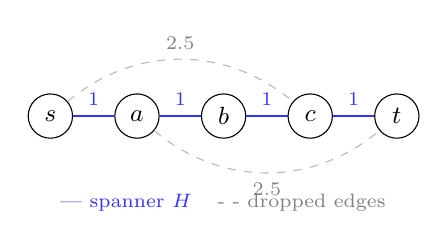
\begin{tikzpicture}[
  nd/.style={circle, draw, fill=white, minimum size=16pt,
             inner sep=0pt, font=\small},
  sp/.style={-, thick, blue!80},
  dr/.style={-, dashed, gray!55},
  lbl/.style={font=\scriptsize, midway}
]
% Five nodes in a line
\node[nd] (s) at (0,   0) {$s$};
\node[nd] (a) at (1.1, 0) {$a$};
\node[nd] (b) at (2.2, 0) {$b$};
\node[nd] (c) at (3.3, 0) {$c$};
\node[nd] (t) at (4.4, 0) {$t$};

% Spanner edges: path s-a-b-c-t, all weight 1
\draw[sp] (s) -- node[lbl, above]{1} (a);
\draw[sp] (a) -- node[lbl, above]{1} (b);
\draw[sp] (b) -- node[lbl, above]{1} (c);
\draw[sp] (c) -- node[lbl, above]{1} (t);

% Chord s-c (weight 2.5): processed 5th; d_H(s,c)=3 <= 3*2.5=7.5 -> DROP
\draw[dr] (s) to[bend left=40]
  node[lbl, above, gray]{2.5} (c);

% Chord a-t (weight 2.5): processed 6th; d_H(a,t)=3 <= 3*2.5=7.5 -> DROP
\draw[dr] (a) to[bend right=40]
  node[lbl, below, gray]{2.5} (t);

% Legend
\node[font=\scriptsize, blue!80, anchor=west] at (0,-1.1)
  {--- spanner $H$};
\node[font=\scriptsize, gray,    anchor=west] at (2.0,-1.1)
  {- - dropped edges};
\end{tikzpicture}
\caption{A 3-spanner of a 5-node graph constructed by the Greedy
algorithm ($k=2$, $\alpha=3$). Edges are processed in
non-decreasing weight order: the four path edges (weight~1) are
added first, building $H = s$-$a$-$b$-$c$-$t$. The two chords
(weight~2.5) are then considered and dropped because
$d_H(s,c) = 3 \leq 3 \times 2.5 = 7.5$ and
$d_H(a,t) = 3 \leq 3 \times 2.5 = 7.5$.}
\label{fig:spanner}
\end{figure}

% ── 4. Implementation ────────────────────────────────────────────
\section{Implementation and Experiment Plan}

Implementation proceeds in three phases:

\begin{enumerate}[leftmargin=*, topsep=2pt, itemsep=1pt]
  \item \textbf{Greedy Spanner:} Sort edges by weight; add each
    edge if the current spanner does not already provide a
    $d \leq \alpha w(u,v)$ path, as described in
    \citet{chimani2022spanner}.
  \item \textbf{Baswana--Sen Spanner:} Execute $k{-}1$ rounds of
    cluster sampling to build a $(2k-1)$-spanner in expected
    $O(km)$ time, as described in \citet{chimani2022spanner}.
  \item \textbf{Evaluation Suite:} Measure and compare both
    algorithms on all benchmark instances from
    Table~\ref{tab:datasets}.
\end{enumerate}

Algorithm~\ref{alg:greedy} describes the Greedy construction.
Algorithm~\ref{alg:bs} describes the Baswana--Sen procedure.

\begin{algorithm}[t]
\caption{Greedy $(2k{-}1)$-Spanner}
\label{alg:greedy}
\begin{algorithmic}[1]
\Require Graph $G=(V,E,w)$, integer $k \geq 1$
\Ensure Subgraph $H$ with stretch $\alpha = 2k-1$
\State Sort $E$ by $w$ in non-decreasing order
\State Initialize $H \leftarrow (V,\,\emptyset)$
\For{each edge $(u,v) \in E$}
  \State $d \leftarrow$ shortest-path dist.\ from $u$ to $v$ in $H$
  \If{$d > (2k-1)\cdot w(u,v)$}
    \State Add $(u,v)$ to $H$
  \EndIf
\EndFor
\State \Return $H$
\end{algorithmic}
\end{algorithm}

\begin{algorithm}[t]
\caption{Baswana--Sen $(2k{-}1)$-Spanner}
\label{alg:bs}
\begin{algorithmic}[1]
\Require Graph $G=(V,E,w)$, integer $k \geq 1$
\Ensure Spanner $H$ with expected $O(n^{1+1/k})$ edges
\State $E_H \leftarrow \emptyset$;\;
       $\mathcal{C} \leftarrow \{\{v\} : v \in V\}$
\For{$i = 1$ \textbf{to} $k-1$}
  \State Sample each cluster centre into $R_i$ w.p.\ $n^{-1/k}$
  \For{each $v \notin R_i$}
    \If{$v$ has a neighbour in a cluster centred at $R_i$}
      \State Add lightest such edge to $E_H$; join that cluster
    \Else
      \State Add all edges from $v$ to its current cluster to $E_H$
      \State Remove $v$ from $\mathcal{C}$
    \EndIf
  \EndFor
  \State $\mathcal{C} \leftarrow$ clusters centred at $R_i$
\EndFor
\State Add all edges within remaining clusters to $E_H$
\State \Return $H = (V, E_H)$
\end{algorithmic}
\end{algorithm}

\subsection{Algorithmic Approach}

For the Greedy spanner, the inner distance query runs Dijkstra
on the current partial spanner $H$.
Because $H$ grows monotonically and early iterations involve a
sparse $H$, this is fast in practice.
The Baswana--Sen algorithm requires only BFS traversals and
adjacency-list lookups, achieving its $O(km)$ bound without any
global distance computation.

\subsection{Evaluation Metrics}

We measure five quantities for each (algorithm, instance, $k$)
triple:

\begin{enumerate}[leftmargin=*, topsep=2pt, itemsep=1pt]
  \item \textbf{Sparseness:} $|E_H|/n$ (edges per vertex).
  \item \textbf{Lightness:}
    $w(E_H)\,/\,w(\mathrm{MST}(G))$.
  \item \textbf{Effective stretch:}
    For small instances ($n \leq 500$), exact
    $\max_{u \neq v}\, d_H(u,v)\,/\,d_G(u,v)$ via all-pairs
    shortest paths. For larger instances, we sample 1,000
    random source--target pairs and report the maximum observed
    ratio as an approximate lower bound on the true stretch.
  \item \textbf{Peak memory:} Measured via Python's
    \texttt{tracemalloc} module at the point of maximum
    allocation during spanner construction.
  \item \textbf{Running time:} Wall-clock time averaged over
    5 runs per instance.
\end{enumerate}

\subsection{Anticipated Technical Challenges}

\textbf{Greedy bottleneck.}
Each edge in the Greedy algorithm triggers a Dijkstra call on
the growing $H$, giving $O(m^2 \log n)$ worst-case time for
dense graphs.
Per \citet{chimani2022spanner}, ADDJS solves all TSPLIB instances
with $n \leq 1{,}200$ within their time limit; we adopt the same
threshold and profile per-instance runtimes to identify our own
practical cutoff on available hardware.

\textbf{Randomness in Baswana--Sen.}
The BS algorithm is randomized; spanner size varies across runs.
We will report means and standard deviations across 10 independent
runs per instance, following the repeated-trial methodology of
\citet{chimani2022spanner}.

% ── 5. Resources ─────────────────────────────────────────────────
\section{Resources Declaration}

Python is the primary language.
Core libraries: NetworkX for graph operations and shortest-path
oracles; NumPy and Matplotlib for data aggregation and
visualization.
Real-world graphs are sourced from the SNAP repository.
Experiments run on personal workstations with standard CPU
configurations.

\begin{table}[t]
\centering
\setlength{\tabcolsep}{3pt}
\begin{tabular}{>{\raggedright\arraybackslash}p{1.85cm}
                >{\raggedright\arraybackslash}p{1.25cm}
                >{\raggedright\arraybackslash}p{1.65cm}
                >{\raggedright\arraybackslash}p{0.9cm}}
\toprule
\textbf{Family} & \textbf{Source} & \textbf{$|V|$ range} & \textbf{$N$} \\
\midrule
Random (ER)    & Synth.    & 10--2000           & 720  \\
TSPLIB         & TSPLIB    & up to 7,397        & 95   \\
Steinlib       & Steinlib  & varies             & 1207 \\
Facebook       & SNAP      & 4,039              & 1    \\
Gnutella       & SNAP      & 6,301              & 1    \\
\bottomrule
\end{tabular}
\caption{Benchmark instances replicating \citet{chimani2022spanner}
plus SNAP extensions. The two largest TSPLIB instances
($n\!=\!5{,}915$ and $n\!=\!7{,}397$) are excluded from Greedy
runs due to runtime constraints, matching the original study.}
\label{tab:datasets}
\end{table}

% ── References ───────────────────────────────────────────────────
\bibliographystyle{plainnat}
\bibliography{refs_spanner}

\end{document}